\documentclass[a4paper,12pt]{article}
\usepackage[utf8]{inputenc}
\usepackage{geometry}
\usepackage{fancyhdr}
\usepackage{amsmath}
\usepackage{wallpaper}
\usepackage{graphicx}
\pagestyle{fancy}
\fancyhf{}
\fancyhead[L]{Solution: LFPy-exercise BNNI 2019}

\begin{document}
\section*{Solution to LFPy-exercise:\\Forward modelling of extracellular potentials}

\paragraph{(i)} This is actually a complicated question, where you in general have to find a balance between False Nagative errors (not registering a spike that is there) and False Positive errors (registering a spike that is not there). The electrode is re-positioned by changing the variable \texttt{elec\_x = np.array([25.])} in the script.  Roughly speaking, the spike becomes difficult to distinguish from the noise at a distance of about 40 $\mu m$ away from the soma (see Figure 1).

%%%%
\begin{figure}[hb]
\centering
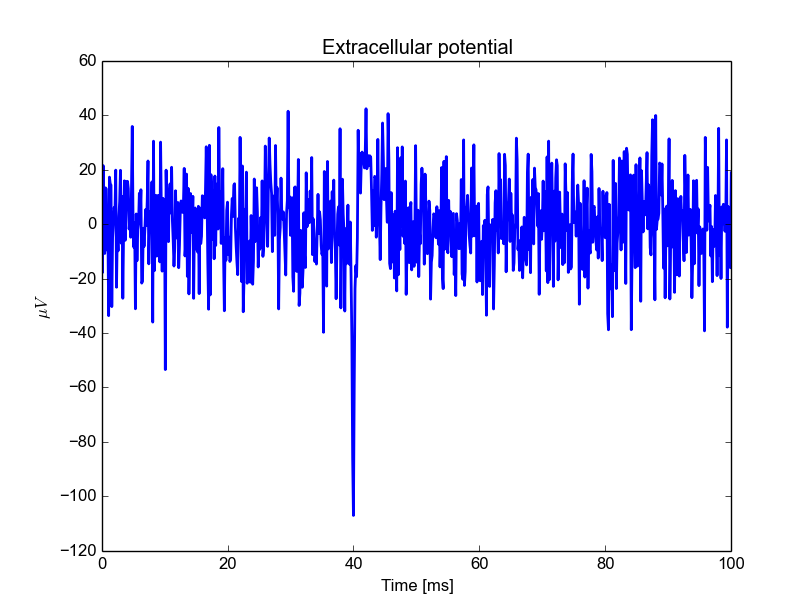
\includegraphics[width=6cm]{spike_30um}
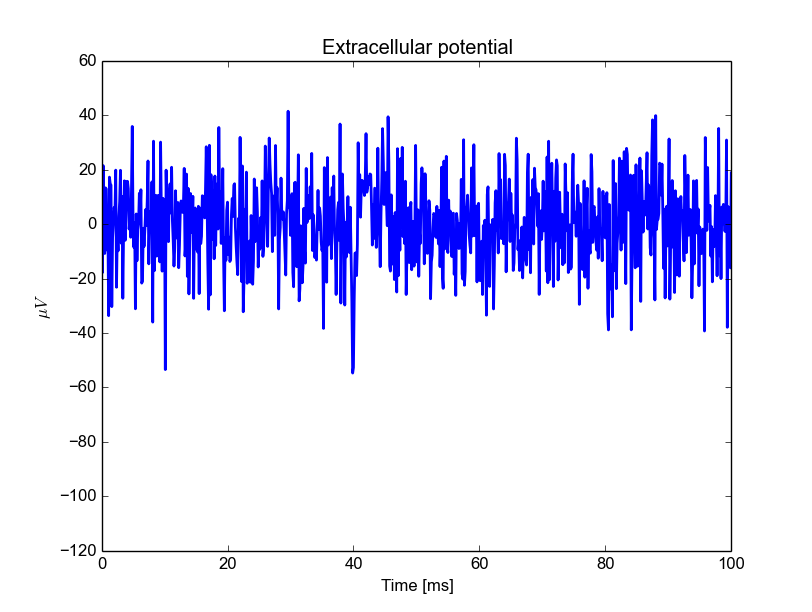
\includegraphics[width=6cm]{spike_40um}
\caption{For white noise with a Root-Mean-Square amplitude of 15 $\mu V$ added to the extracellular signal,
the spike is visible in the extracellular medium 30 $\mu m$ (left) to 40 $\mu m$ (right) away from the soma.}
\end{figure}
%%%%

\paragraph{(iia)} The plot is simply generated by un-commenting the line \texttt{dense\_2D\_LFP(cell)} in the script. It should produce an output as in the left panel of Figure 2.

\paragraph{(iib)} The synapse position is set by changing the argument \texttt{synaptic\_y\_pos} in the script. In Figure 2 we can see that a synapse in the soma (left panel) or distal apical dendrite (right panel) gives a dipole-like LFP, while a synapse in the middle of the apical dendrite gives a multipolar LFP (middle panel). 

\paragraph{(iic)} Any higher order multipole will generally decay more rapid with distance than a dipole, implying that somatic and distal apical synapses can be expected to have larger contributions to the LFP than the input to the center of the apical dendrite. 

%%%%
\begin{figure}[hb]
\centering
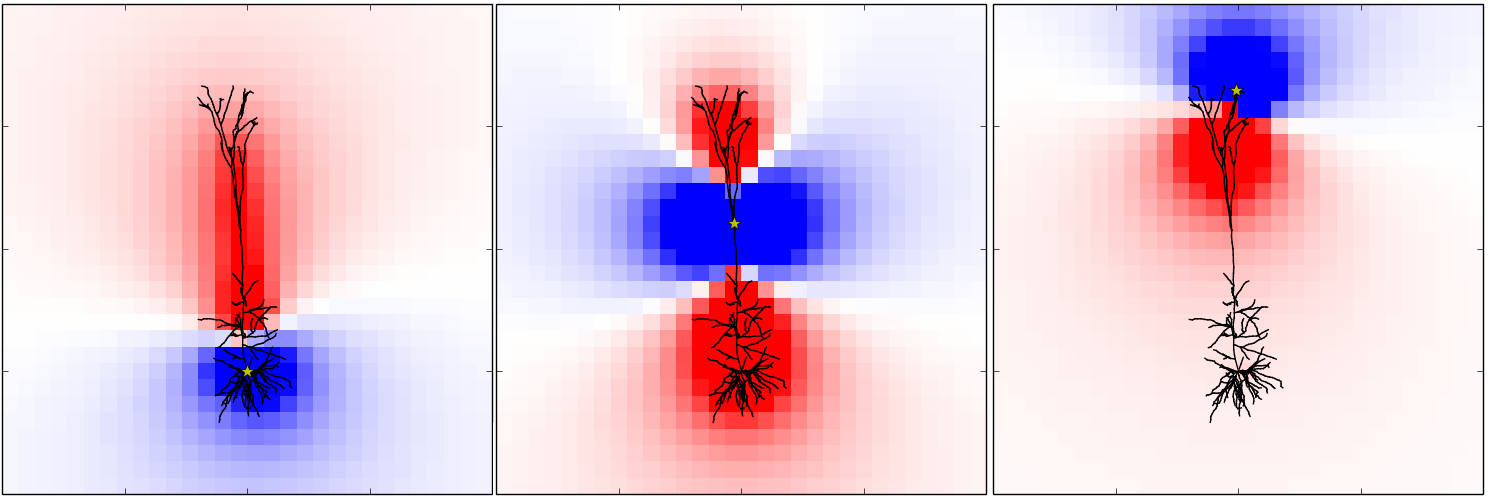
\includegraphics[width=10cm]{grid}
\caption{The amplitude of the LFP at a time shortly after the synaptic input has arrived either to the soma (left), to the middle of the apical dendrite (center), or to the distal apical tuft (right). The color scale is the same in 
all figures.}
\end{figure}
%%%%

\paragraph{(iii) [Optional]} Cells that are have sperical symmetry, like the interneuron, will not get as clean dipole LFP, and this will lead to a more rapid decay of signal power with distance, decreasing their importance for the LFP.
See paper by Lindèn et al. (2010) that is cited in the exercise.
\end{document}
